\documentclass[a4paper]{article}

\usepackage[14pt]{extsizes}
\usepackage[T2A]{fontenc}
\usepackage[russian]{babel}

\usepackage[left=20mm, top=15mm, right=15mm, bottom=20mm]{geometry}
\usepackage{listings}
\usepackage{xcolor}
\usepackage{tikz}
\usetikzlibrary{shapes.geometric, arrows.meta, positioning, calc, arrows, shapes.misc}
\usepackage{graphicx}
\usepackage{amsmath, amssymb} % For equations
\usepackage{booktabs} % For better tables
\usepackage{pgfplots} % For plotting graphs
\usepackage{caption} % For captioning tables and figures
\usepackage{float} % For precise float placement (images, tables)
\usepackage[hidelinks]{hyperref} % For table of contents to be clickable
\usepackage{bookmark}
\usepackage{multirow}
\usepackage{array}
\usepackage{cancel}
\usepackage{placeins}
\usepackage{enumitem}
\pgfplotsset{compat=1.17}
\usepackage{circuitikz}
\usetikzlibrary{decorations.markings} % For custom arrow positioning

% -----------------------------------------------------

% % listing for programming code blocks
\lstset{
	language=C++,                 % Programming language
	basicstyle=\ttfamily\normalsize, % Adjust font size
	keywordstyle=\color{blue},    % Style for keywords
	stringstyle=\color{red},      % Style for strings
	commentstyle=\color{gray},   % Style for comments
	morecomment=[l][\color{magenta}]{\#}, % Special comment style
	breaklines=true,              % Line breaking in long lines
	numbers=left,                 % Line numbering on the left
	numberstyle=\tiny\color{gray},% Style for line numbers
	frame=single,                 % Code frame
	showstringspaces=false        % Don't show spaces in strings
}

% % tikz styles for flowcharts
\tikzset{
	startstop/.style={
			rectangle,
			rounded corners,
			minimum width=3cm,
			minimum height=1cm,
			text centered,
			draw=black,
			fill=red!30
		},
	io/.style={
			trapezium,
			trapezium left angle=70,
			trapezium right angle=110,
			minimum width=3cm,
			minimum height=1cm,
			text centered,
			draw=black,
			fill=blue!30
		},
	process/.style={
			rectangle,
			minimum width=3cm,
			minimum height=1cm,
			text centered,
			draw=black,
			fill=orange!30
		},
	decision/.style={
			diamond,
			aspect=2,
			minimum width=3cm,
			text centered,
			draw=black,
			fill=green!30
		},
	arrow/.style={
			thick,
			->,
			>=stealth
		},
	prep/.style={
			chamfered rectangle,
			chamfered rectangle xsep=2cm,
			draw,
			thick,
			minimum width=5cm,
			minimum height=1cm,
			text centered,
			text width=2.5cm,
			font=\small,
			fill=yellow!30
		},
}


\begin{document}

% Title page
\begin{center}
	\vspace{1cm}
	\large{Университет ИТМО}\\
	\large{Факультет программной инженерии и компьютерной техники}\\
	\vspace{4cm}
	\Large{\textbf{Лабораторная работа №1\\}}
	\vspace{0.3cm}
	\large{\textbf{<<Введение в проектирование цифровых интегральных схем>>\\}}
	\vspace{-0.3cm}
	\begin{center}
		\large{по дисциплине <<Функциональная схемотехника>>}
	\end{center}
	\vspace{3cm}
\end{center}
\normalsize{
	\begin{flushright}
		Выполнили:
		\par
		Студенты группы P3331
		\par
		Дворкин Борис Александрович
		\par
		Краков Кирилл Константинович
		\par
		\textbf{Вариант: 1}
		\par
		\vspace{1cm}
		Преподаватель:
		\par
		Васильев Сергей Евгеньевич
	\end{flushright}
}\\
\vspace{6cm}
\begin{center} г. Санкт-Петербург
	\par
	2024 г.
\end{center}

\thispagestyle{empty}

\newpage
\pagestyle{plain}
\setcounter{page}{1}

% -------------------------------

% autogenerated table of contents
\linespread{0.9}
\tableofcontents
\linespread{1}

% -------------------------------

\newpage
\section*{Цель работы}
\addcontentsline{toc}{section}{Цель работы}
\begin{enumerate}
	\item Получить базовые знания о принципах построения цифровых интегральных схем с использованием технологии \textbf{комплементарной структуры металл -- оксид -- полупроводник} (КМОП).
	\item Познакомиться с технологией \textbf{SPICE-моделирования} схем на транзисторах.
	\item Получить навыки описания схем \textbf{базовых операционных элементов} (БОЭ) комбинационного типа на вентильном уровне с использованием языка описания аппаратуры \textbf{Verilog HDL}.
\end{enumerate}


% -------------------------------

\section*{Задание в соответствии с вариантом}
\addcontentsline{toc}{section}{Задание в соответствии с вариантом}
В рамках лабораторной работы №1 было выдано следующее задание:

\begin{itemize}
    \item Логический базис: \textbf{NOR}
    \item Базовый операционный элемент (БОЭ): \textbf{Демультиплексор «1 в 4»}
\end{itemize}

Целью работы является проектирование цифровой интегральной схемы с использованием технологии КМОП на транзисторном уровне, а также моделирование и тестирование её работы с использованием среды LTspice. В дополнение, необходимо разработать описание БОЭ на вентильном уровне с применением языка Verilog HDL и провести его моделирование в среде Vivado Design Suite.

Задание включает два основных этапа:
\begin{enumerate}
    \item Построение схемы вентиля \textbf{NOR} на полевых транзисторах и моделирование его работы в LTspice, а затем использование его для создания демультиплексора «1 в 4».
    \item Описание схемы демультиплексора на языке Verilog HDL, создание тестового окружения и проведение моделирования в Vivado.
\end{enumerate}


% -------------------------------

\stepcounter{section}
\section*{Часть 1}
\addcontentsline{toc}{section}{Часть 1}
\subsection{Схема разработанного вентиля}
\subsubsection{Описание}
Разработанный NOR-вентиль реализован на КМОП-транзисторах и состоит из пары p-канальных (\( M_1 \), \( M_2 \)) и n-канальных (\( M_3 \), \( M_4 \)) транзисторов. Вентиль выдаёт логическую $"1"$ на выходе \( \text{Out} \), только когда оба входа \( A \) и \( B \) находятся в $"0"$. При подаче $"1"$ на любой из входов nMOS транзисторы подключают выход к земле (GND), устанавливая $"0"$ на выходе, выполняя функцию NOR.

\subsubsection{Схема NOR-вентиля}
\begin{figure}[H]
	\centering
	\begin{circuitikz}[european, scale=1.5, transform shape]
		\draw (0,0)
		-- (4,0) to[short, *-] (4,0)
		-- (10,0) node[right] {$\small V_{\text{\scriptsize DD}}$};

		\draw (0,-5.5)
		-- (4,-5.5) to[short, *-] (4,-5.5)
		-- (10,-5.5) node[right] {\small GND};

		\draw (4,0) -- (4, -0.23)
		++(0, -0.77) node[pmos,emptycircle]{\small $M_1$} (4, -1.5)
		++ (0, -1.05) node[pmos,emptycircle]{\small $M_2$} (4,-3)
		++(0, -0.325) --(4, -3.41)
		++(0, -1.055) node[nmos,emptycircle]{\small $M_3$} (4, -5)
		++(0, -0.24) -- (4, -5.5);

		\draw
		(1, -1) node[left]{\small $A$}
		-- (3.015, -1);

		\draw (2.5, -1)
		to [short, *-] (2.5, -1)
		-- (2.5, -2.41)
		++ (0, -0.28)
		-- (2.5, -3.55)
		-- (3.861, -3.55) ++(0.139, 0) node[jump crossing] ++(0.14, 0)
		-- (5.3, -3.55)
		-- (5.3, -4.275)
		-- (5.525, -4.275);

		\draw
		(1, -2.55) node[left]{\small $B$}
		-- (2.36, -2.55) ++(0.14, 0) node[jump crossing] (2.55, -2.55)
		++(0.14, 0) -- (3.016, -2.55);

		\draw (2, -2.55)
		to [short, *-] (2, -2.55)
		-- (2, -4.465) -- (3.02, -4.465);

		\draw (6.5, -5.5)
		to [short, *-] (6.5, -5.5)
		-- (6.5, -5.05)
		++(0, 0.775) node[nmos,emptycircle]{\small $M_4$} (6.5, -3.5)
		-- (6.5, -2.75)
		to[short, *-] (6.5, -2.75);

		\draw (5, -2.75)
		-- (10, -2.75) node[right] {\small Out};

		\draw (4, -3.2)
		to[short, *-] (4, -3.2)
		-- (5, -3.2)
		-- (5, -2.75);

	\end{circuitikz}
	\caption{NOR вентиль на nMOS и pMOS транзисторах}
\end{figure}


\subsection{Символ вентиля}
\begin{figure}[H]
	\centering
	\begin{circuitikz}[european, scale=2.5, transform shape]
		\draw[thick] node[ieeestd nor port] (N) {};
		\draw[thick] (N.up) -- ++(0, 0.3) ++(0, 0.2) node[up] {\scriptsize $V_{\text{DD}}$}
		\draw[thick] (N.left) ++ (-0.3, 0.3) node[left] {\scriptsize $A$}
		\draw[thick] (N.left) ++ (-0.3, -0.3) node[left] {\scriptsize $B$}
		\draw[thick] (N.N-not) ++ (1, 0) node[right] {\scriptsize Out}
	\end{circuitikz}
	\caption{символ NOR вентиля на nMOS и pMOS транзисторах}
\end{figure}


\subsection{Схема тестирования}
\begin{figure}[H]
	\centering
	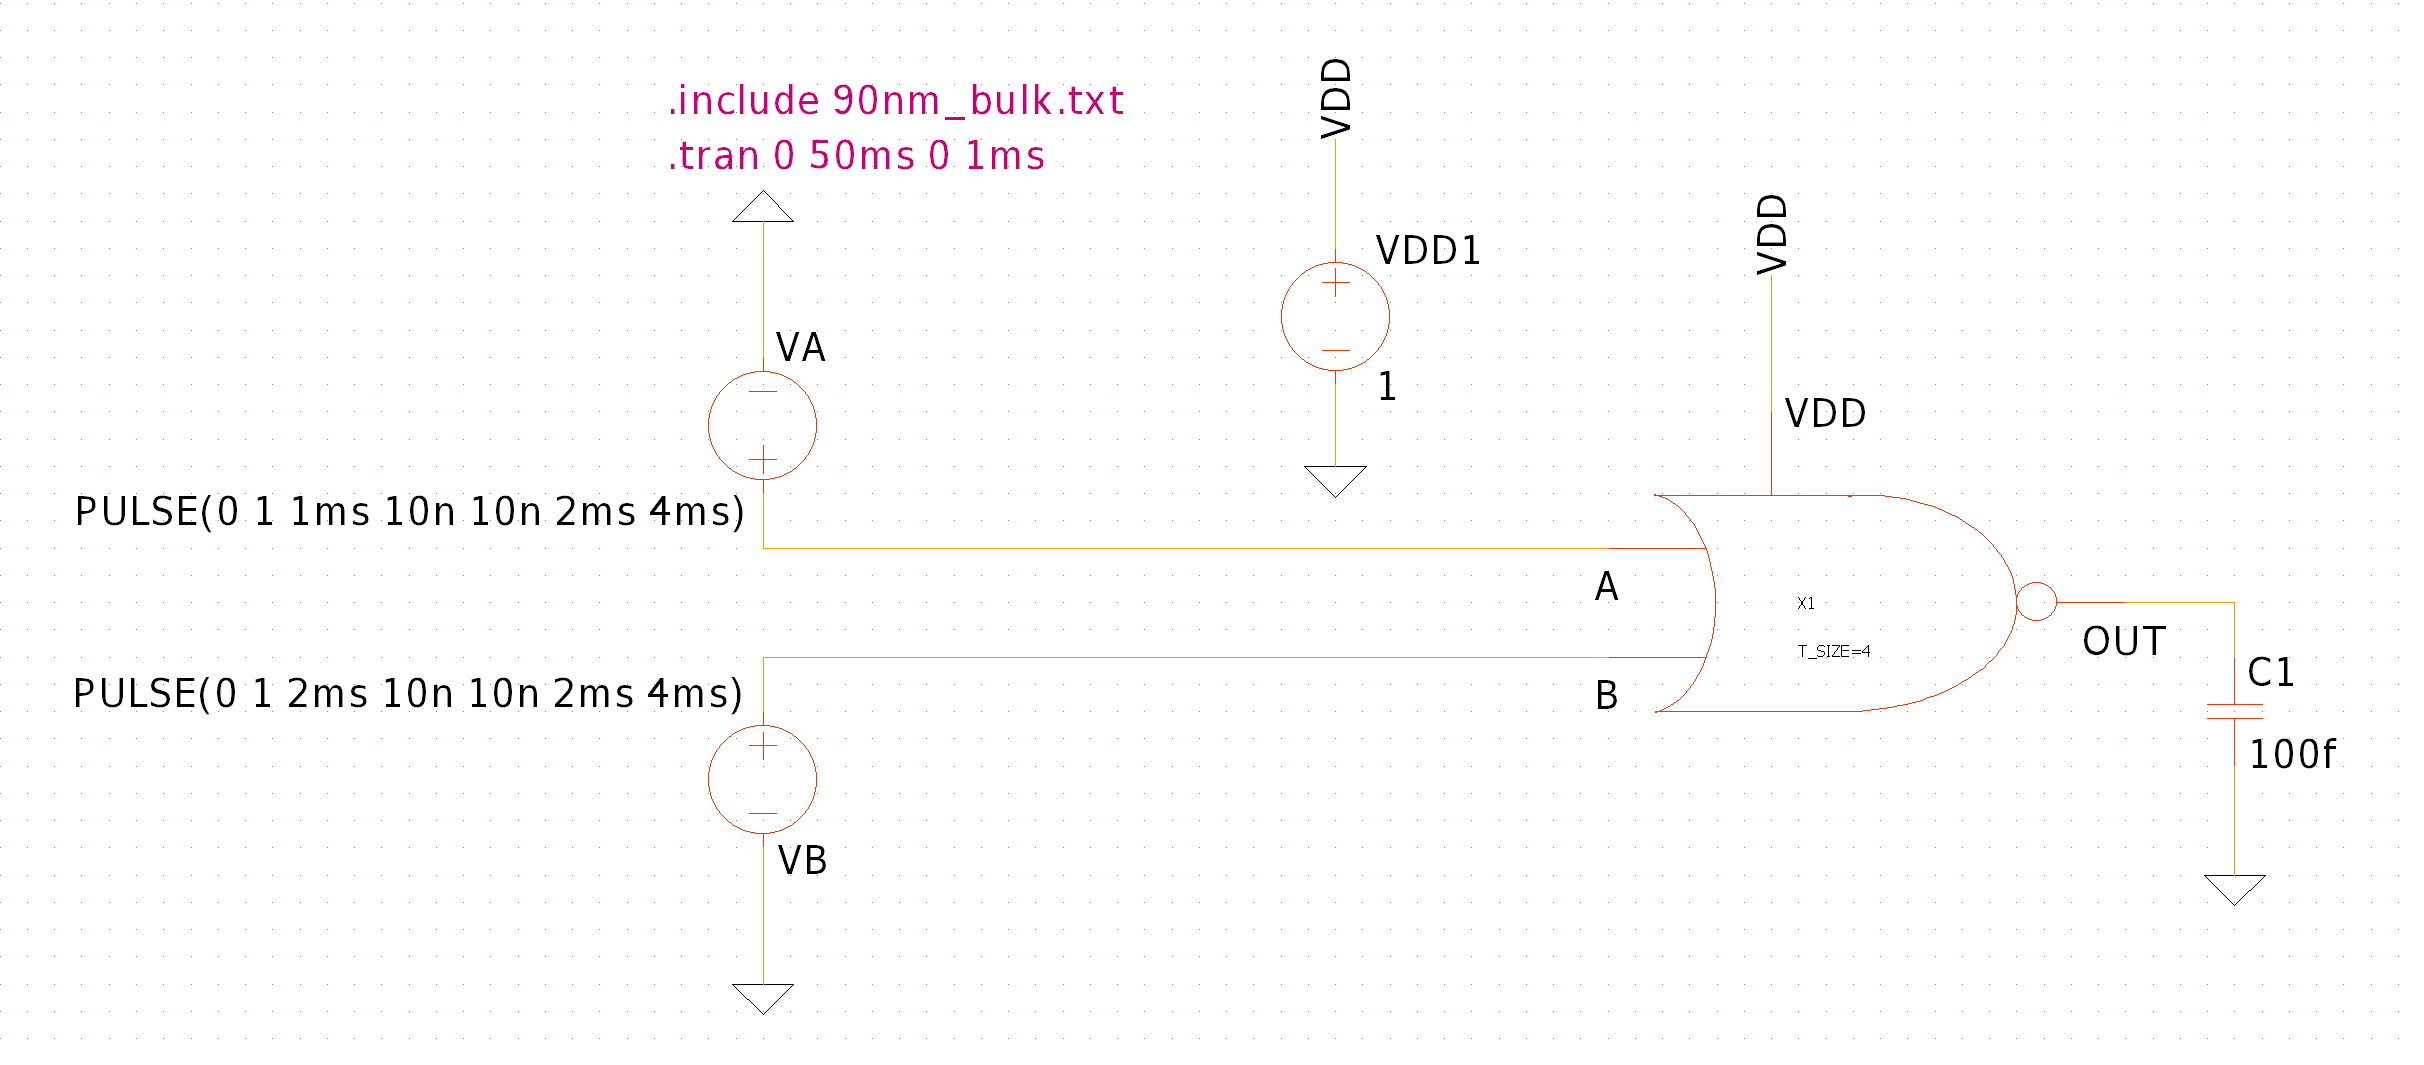
\includegraphics[width=1\textwidth]{../data/test_cmos_nor}
	\caption{Схема тестирования разработанного NOR-вентиля}
\end{figure}


\subsection{Временная диаграмма тестирования вентиля}
\setlength{\columnsep}{1cm}

\begin{multicols}{2}
	Тестируемый NOR-элемент должен соответствовать следующей таблице истинности.

	Временная диаграмма на Рисунке 4 показывает изменение напряжений на входах \( A \), \( B \) и выходе \( \text{Out} \) во времени, подтверждая правильность работы NOR-элемента.

	\columnbreak

	\noindent
	\renewcommand{\arraystretch}{1.33}
	\raggedright
	\begin{tabular}{|>{\centering\arraybackslash}p{1.2cm}|>{\centering\arraybackslash}p{1.2cm}|>{\centering\arraybackslash}p{1.6cm}|}
		\hline
		A & B & Out \\
		\hline
		0 & 0 & 1   \\
		0 & 1 & 0   \\
		1 & 0 & 0   \\
		1 & 1 & 0   \\
		\hline
	\end{tabular}

\end{multicols}

\begin{figure}[H]
	\centering
	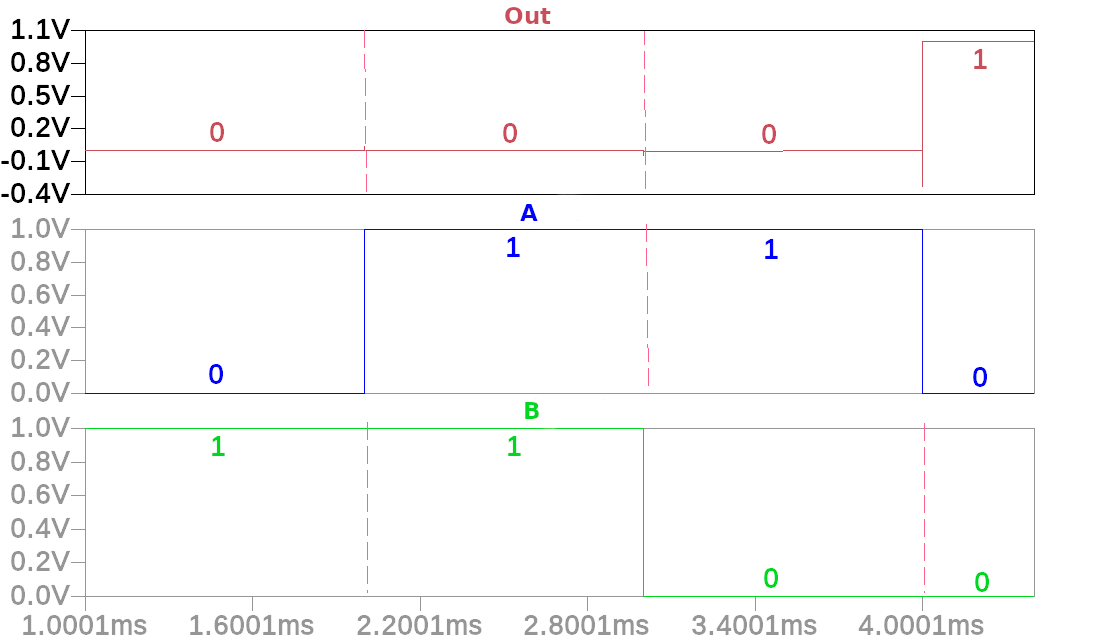
\includegraphics[width=0.8\textwidth]{../data/test_cmos_nor_time}
	\caption{Временная диаграмма напряжений на A, B, Out}
\end{figure}


\subsection{Результат измерения задержки распространения сигнала через вентиль}
Задержка распространения сигнала была измерена на временной диаграмме (см. Рис. 5 с увеличенным масштабом). Измерение проводилось от момента изменения входного сигнала до достижения выходным сигналом 50\% от напряжения \( V_{DD} \). Рассчитанная задержка:

\[
	t_{pd} = t_{out} - t_{in} = 4.00003551 - 4.000009788 = 25.722 \, \text{нс}
\]

\begin{figure}[H]
	\centering
	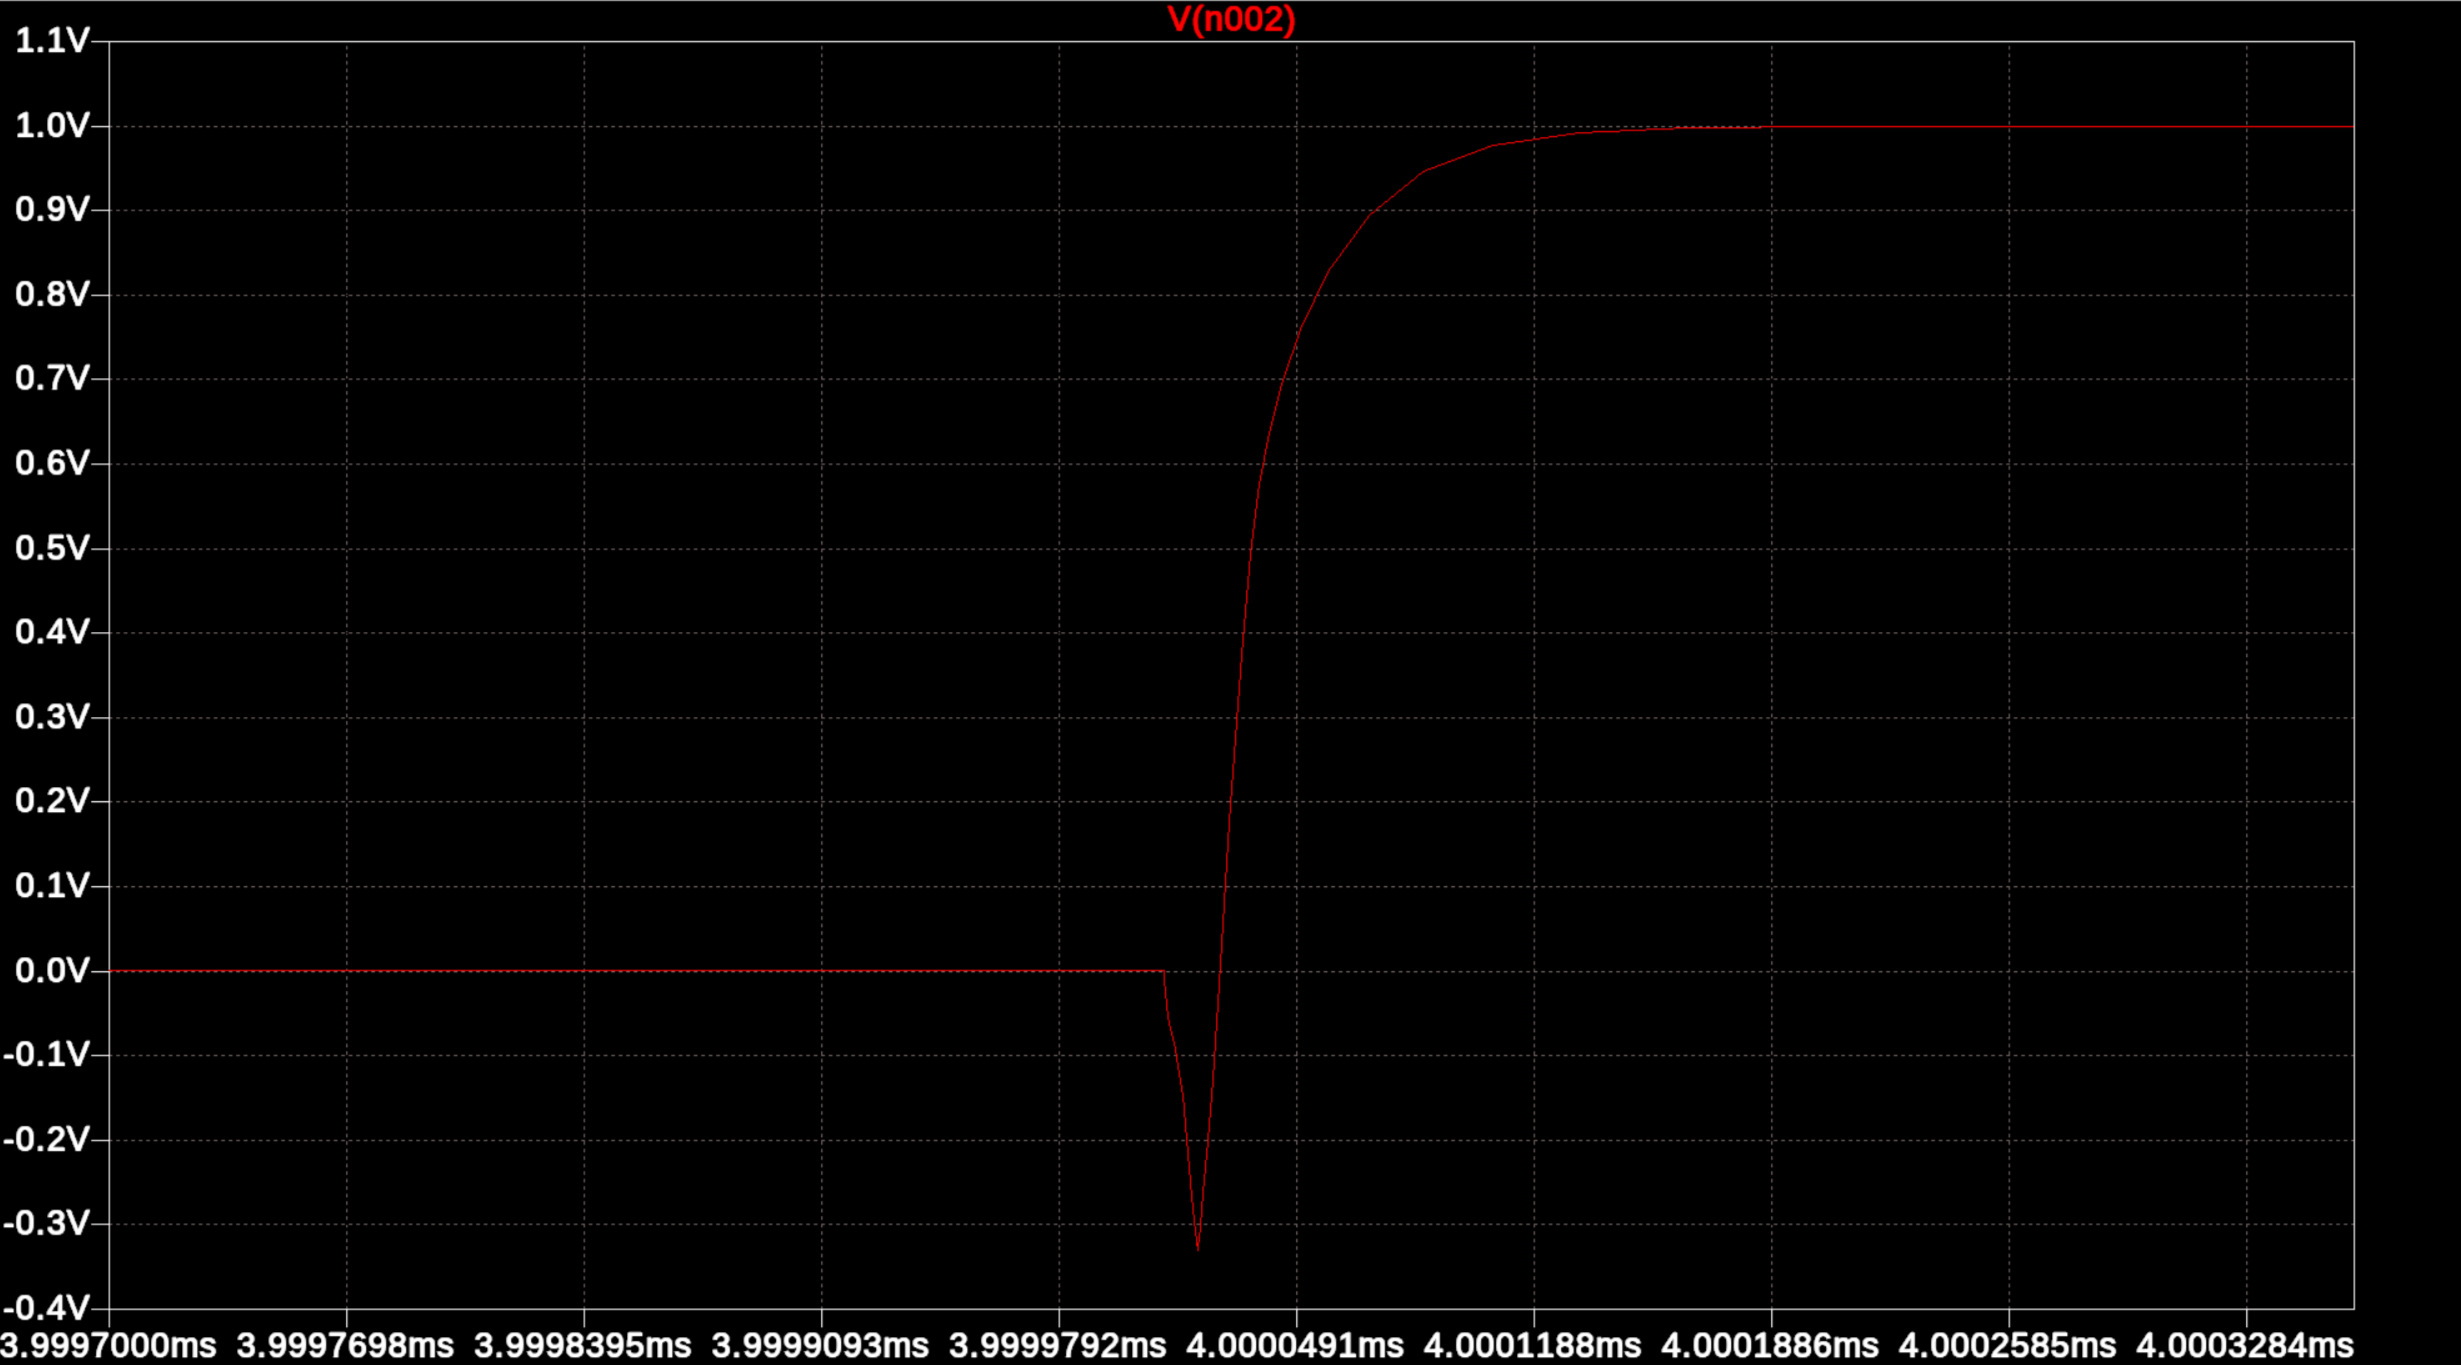
\includegraphics[width=1\textwidth]{../data/t_delay_zoomed}
	\caption{Увеличенная временная диаграмма напряжений на Out}
\end{figure}

\subsection{Максимальная частота работы вентиля}
Максимальная частота работы вентиля рассчитывается по формуле:

\[
	f_{max} = \frac{1}{2 \cdot t_{pd}}
\]

Подставив \( t_{pd} = 25.722 \, \text{нс} \), получаем:

\[
	f_{max} = \frac{1}{2 \cdot 25.722 \cdot 10^{-9}} = 19,439 \, \text{МГц}
\]

Следовательно, максимальная частота работы вентиля составляет \( 19,439 \, \text{МГц} \).

\subsection{Схема разработанного БОЭ}
% \begin{figure}[H]
% 	\centering
% 	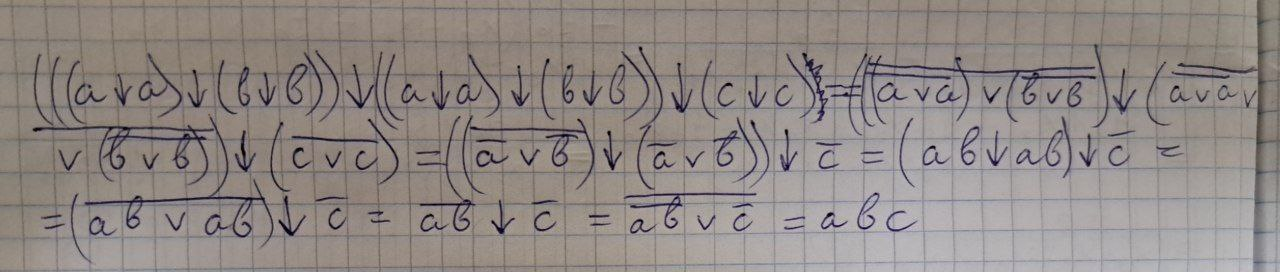
\includegraphics[width=1\textwidth]{../data/formula}
% 	\caption{Вывод схемы БОЭ}
% \end{figure}

\subsubsection{Вывод схемы БОЭ}

Для каждого выхода \( Z_i \) на основе таблицы истинности строим логическое выражение в базисе ИЛИ-НЕ.

### Выражение для \( Z_0 \):
\[
	\begin{gathered}
		Z_0 = \overline{S_1} \cdot \overline{S_0} \cdot Y = \overline{(S_0 \vee S_1) \vee \overline{Y}} = (\overline{\overline{S_0 \vee S_1}}) \vee \overline{Y} \\
		Z_0 = ((S_0 \downarrow S_1) \downarrow (S_0 \downarrow S_1)) \downarrow (Y \downarrow Y)
	\end{gathered}
\]

### Выражение для \( Z_1 \):
\[
	\begin{gathered}
		Z_1 = \overline{S_1} \cdot S_0 \cdot Y = \overline{(S_1 \vee \overline{S_0}) \vee \overline{Y}} = (\overline{S_1 \vee \overline{S_0}}) \vee \overline{Y} \\
		Z_1 = ((S_1 \downarrow (S_0 \downarrow S_0)) \downarrow (S_1 \downarrow (S_0 \downarrow S_0))) \downarrow (Y \downarrow Y)
	\end{gathered}
\]

### Выражение для \( Z_2 \):
\[
	\begin{gathered}
		Z_2 = S_1 \cdot \overline{S_0} \cdot Y = \overline{(\overline{S_1} \vee S_0) \vee \overline{Y}} = (\overline{\overline{S_1} \vee S_0}) \vee \overline{Y} \\
		Z_2 = (((S_1 \downarrow S_1) \downarrow S_0) \downarrow ((S_1 \downarrow S_1) \downarrow S_0)) \downarrow (Y \downarrow Y)
	\end{gathered}
\]

### Выражение для \( Z_3 \):
\[
	\begin{gathered}
		Z_3 = S_1 \cdot S_0 \cdot Y = \overline{(\overline{S_1} \vee \overline{S_0}) \vee \overline{Y}} = (\overline{\overline{S_1} \vee \overline{S_0}}) \vee \overline{Y} \\
		Z_3 = (((S_1 \downarrow S_1) \downarrow (S_0 \downarrow S_0)) \downarrow ((S_1 \downarrow S_1) \downarrow (S_0 \downarrow S_0))) \downarrow (Y \downarrow Y)
	\end{gathered}
\]

Таким образом, конечные формулы для каждого \( Z_i \) выражены в базисе ИЛИ-НЕ, что соответствует структуре демультиплексора 1 в 4 на базе логического элемента NOR.

Реализация этих логических выражений с использованием NOR-вентиля выглядит следующим образом:

1. Для инверсии сигналов \( S_1 \) и \( S_0 \) используются NOR-вентиля с одинаковыми входами:
\[
	\overline{S_0} = NOR(S_0, S_0), \quad \overline{S_1} = NOR(S_1, S_1)
\]

2. Логические операции для каждого выхода можно развернуть через NOR следующим образом:

\[
	Z_0 = NOR(NOR(NOR(S_1, S_0), NOR(S_1, S_0)), NOR(Y, Y))
\]
\[
	Z_1 = NOR(NOR(NOR(S_1, \overline{S_0}), NOR(S_1, \overline{S_0})) , NOR(Y, Y))
\]
\[
	Z_2 = NOR(NOR(NOR(\overline{S_1}, S_0), NOR(\overline{S_1}, S_0)) , NOR(Y, Y))
\]
\[
	Z_3 = NOR(NOR(NOR(\overline{S_1}, \overline{S_0}), NOR(\overline{S_1}, \overline{S_0})) , NOR(Y, Y))
\]

Таким образом, каждый выход \( Z_i \) активен при соответствующей комбинации управляющих сигналов \( S_1, S_0 \), что реализует функцию демультиплексора на базе NOR-вентиля.

\subsubsection{Схема БОЭ}

\begin{figure}[H]
	\centering
	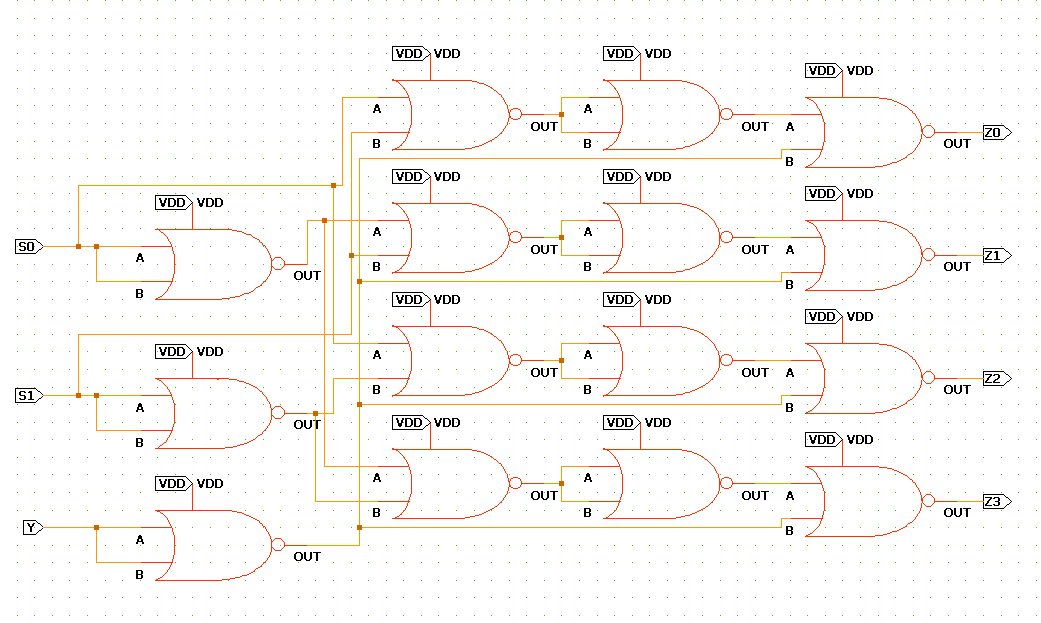
\includegraphics[width=1\textwidth]{../data/demultiplexer_1_to_4}
	\caption{Демультиплексор «1 в 4»}
\end{figure}


\subsection{Символ разработанного БОЭ}
\begin{figure}[H]
	\centering
	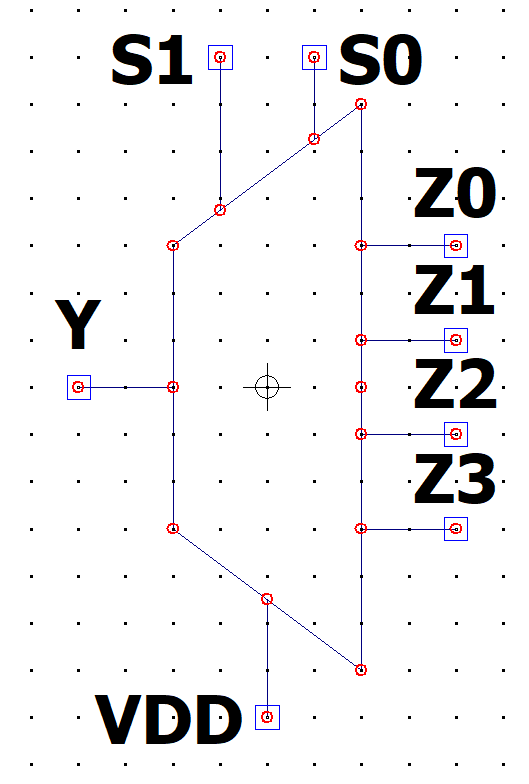
\includegraphics[width=0.4\textwidth]{../data/demux}
	\caption{Символ Демультиплексора <<1 в 4>>}
\end{figure}


\subsection{Схема тестирования разработанного БОЭ}
\begin{figure}[H]
	\centering
	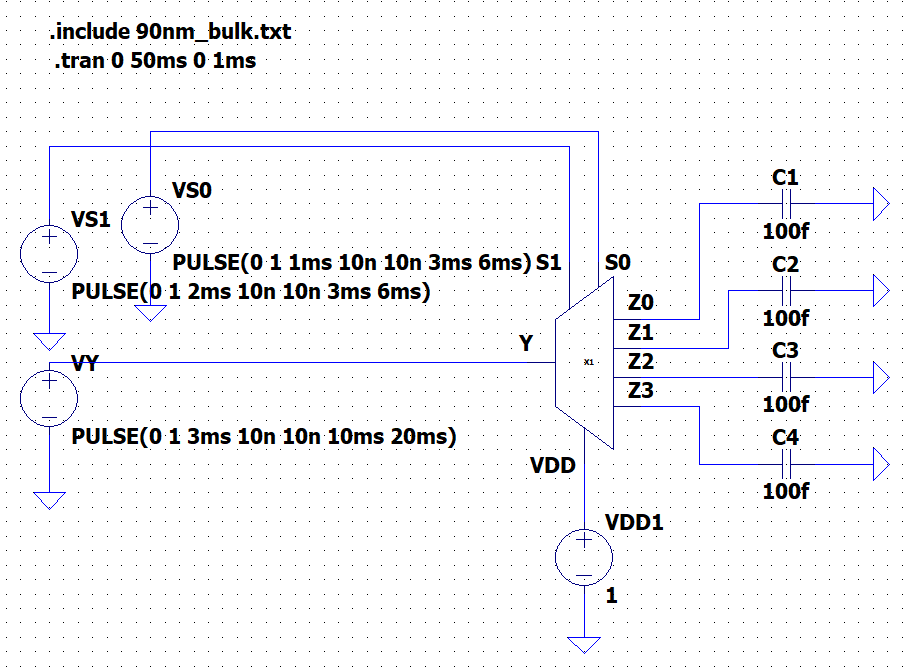
\includegraphics[width=1\textwidth]{../data/boe-testing}
	\caption{Схема тестирования Демультиплексора <<1 в 4>>}
\end{figure}


\subsection{Временная диаграмма тестирования БОЭ}
\setlength{\columnsep}{1cm}

\begin{multicols}{2}
	Тестируемый демультиплексор 1-в-4 должен соответствовать следующей таблице истинности, где \( Y \) — вход, \( S_1 \) и \( S_2 \) — управляющие сигналы, а \( Z_0 \), \( Z_1 \), \( Z_2 \) и \( Z_3 \) — выходы.

	Временная диаграмма на Рисунке 10 показывает изменение напряжений на входах \( Y \), \( S_1 \), \( S_2 \) и выходах \( Z_0 \), \( Z_1 \), \( Z_2 \), \( Z_3 \) во времени, подтверждая правильность работы демультиплексора.

	\columnbreak

	\noindent
	% \vspace*{0.1cm}
	\renewcommand{\arraystretch}{1.12}
	\raggedright
	\begin{tabular}{|>{\centering\arraybackslash}p{0.8cm}|>{\centering\arraybackslash}p{0.8cm}|>{\centering\arraybackslash}p{0.8cm}|>{\centering\arraybackslash}p{0.8cm}|>{\centering\arraybackslash}p{0.8cm}|>{\centering\arraybackslash}p{0.8cm}|>{\centering\arraybackslash}p{0.8cm}|}
		\hline
		$S_1$ & $S_2$ & $Y$ & $Z_0$ & $Z_1$ & $Z_2$ & $Z_3$ \\
		\hline
		0     & 0     & 1   & 1     & 0     & 0     & 0     \\
		0     & 1     & 1   & 0     & 1     & 0     & 0     \\
		1     & 0     & 1   & 0     & 0     & 1     & 0     \\
		1     & 1     & 1   & 0     & 0     & 0     & 1     \\
		\hline
		0     & 0     & 0   & 0     & 0     & 0     & 0     \\
		0     & 1     & 0   & 0     & 0     & 0     & 0     \\
		1     & 0     & 0   & 0     & 0     & 0     & 0     \\
		1     & 1     & 0   & 0     & 0     & 0     & 0     \\
		\hline
	\end{tabular}

\end{multicols}

\begin{figure}[H]
	\centering
	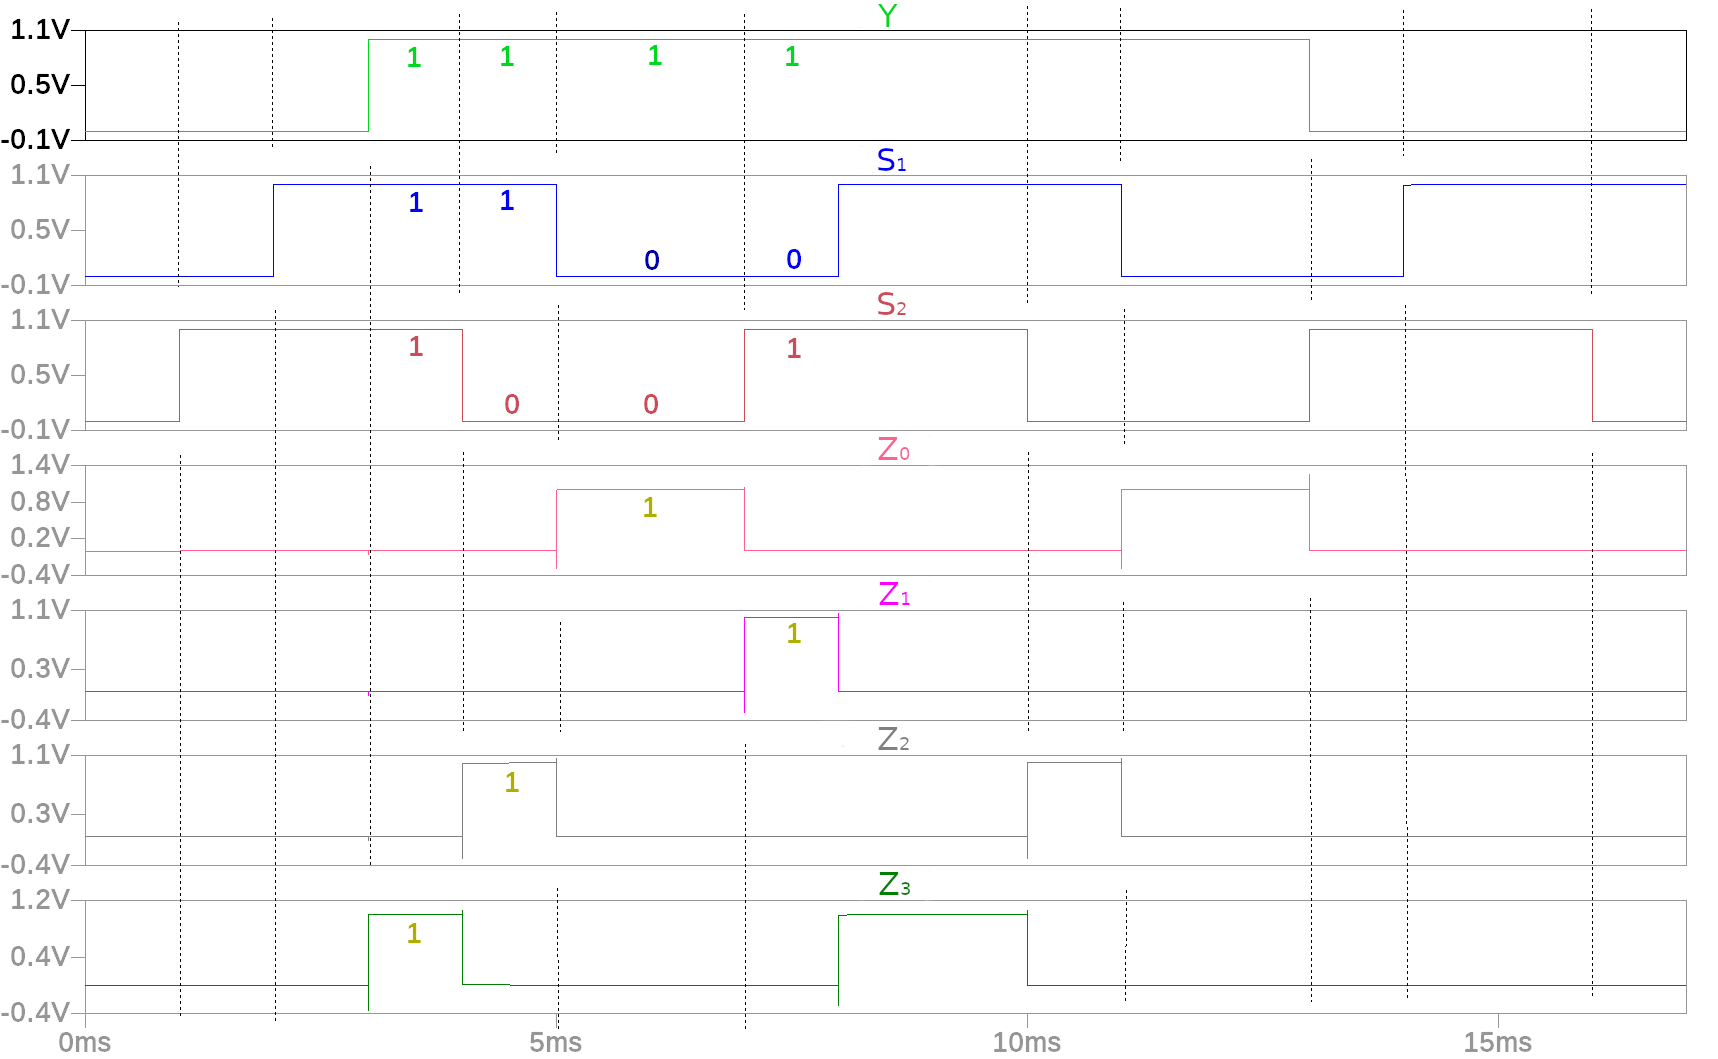
\includegraphics[width=1\textwidth]{../data/test_boe_time}
	\caption{Временная диаграмма напряжений на $Z_0, Z_1, Z_2, Z_3, S_1, S_2, Y$}
\end{figure}


\subsection{Результат измерения задержки распространения сигнала через БОЭ}
Задержка распространения сигнала была измерена на временной диаграмме (см. Рис. 10 с увеличенным масштабом). Измерение проводилось от момента изменения входного сигнала до достижения выходным сигналом 50\% от напряжения \( V_{DD} \). Рассчитанная задержка:

\[
	t_{pd} = t_{out} - t_{in} = 4.0000358 - 4.00001 = 25.8 \, \text{нс}
\]

\begin{figure}[H]
	\centering
	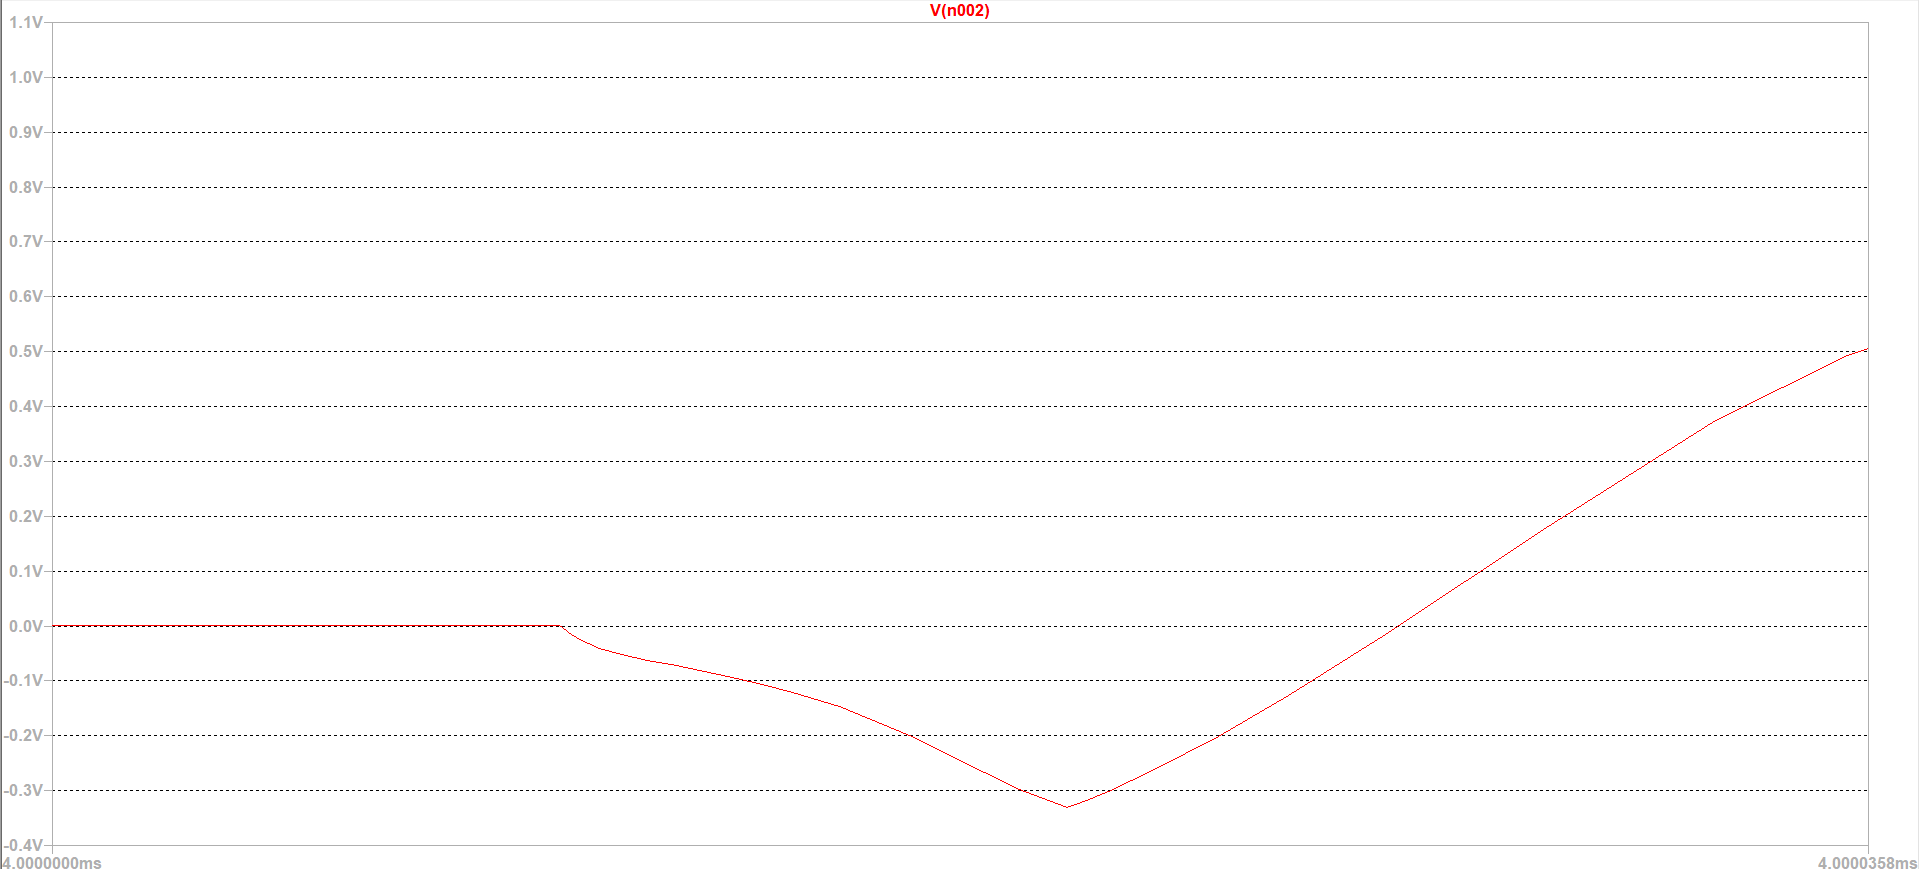
\includegraphics[width=1\textwidth]{../data/test_boe_time_zoomed}
	\caption{Увеличенная временная диаграмма напряжений на Out}
\end{figure}

\subsection{Максимальная частота работы БОЭ}
Максимальная частота работы Демультиплексора <<1 в 4>> рассчитывается по формуле:

\[
	f_{max} = \frac{1}{2 \cdot t_{pd}}
\]

Подставив \( t_{pd} = 25.722 \, \text{нс} \), получаем:

\[
	f_{max} = \frac{1}{2 \cdot 0.0000258 \cdot 10^{-3}} = 19,379 \, \text{МГц}
\]

Следовательно, максимальная частота работы Демультиплексора <<1 в 4>> составляет \( 19,379 \, \text{МГц} \).


% -------------------------------

\section*{Часть 2}
\addcontentsline{toc}{section}{Часть 2}
\subsection{Код разработанного модуля БОЭ}
\subsubsection{Описание}

Код выполнен на языке \textbf{System Verilog} — расширенном Verilog HDL, созданном в 2005 г. Обозначения $[N:N]$ — это так называемые \textit{векторы}, которые используются для задания многобитных сигналов. В System Verilog векторы представляют собой массивы, каждый бит которых может быть обращен и использован в вычислениях. Например, $[3:0]$ обозначает 4-битный вектор, где биты нумеруются от 3 до 0.

В данном коде представлен демультиплексор 1 к 4, реализованный на уровне логических вентилей. Основная функция демультиплексора заключается в том, чтобы передать входной сигнал \textbf{y} на один из четырёх выходов \textbf{z[3:0]} в зависимости от значения управляющего сигнала \textbf{s[1:0]}.

\subsubsection{Программная реализация на System Verilog}

\begin{lstlisting}
module demultiplexer_1_to_4(
    input logic y,
    input logic [1:0] s,
    output logic [3:0] z
    );

    // first lvl
    wire not_s1, not_s0, not_y;

    nor (not_s0, s[0], s[0]);
    nor (not_s1, s[1], s[1]);
    nor (not_y, y, y);
    
    // second lvl
    wire x1, x2, x3, x4;
    nor(x1, s[0], s[1]);
    nor(x2, not_s0, s[1]);
    nor(x3, s[0], not_s1);
    nor(x4, not_s0, not_s1);
    
    // third lvl
    wire not_x1, not_x2, not_x3, not_x4;
    nor (not_x1, x1, x1);
    nor (not_x2, x2, x2);
    nor (not_x3, x3, x3);
    nor (not_x4, x4, x4);
    
    // fourth lvl
    nor (z[0], not_x1, not_y);
    nor (z[1], not_x2, not_y);
    nor (z[2], not_x3, not_y);
    nor (z[3], not_x4, not_y);
endmodule
\end{lstlisting}


\subsection{Код разработанного тестового окружения БОЭ}
\subsubsection{Программная реализация на System Verilog}

В данном коде представлен тестовый модуль для демультиплексора 1 к 4, написанный на языке \textbf{System Verilog}. Этот тестовый модуль (\textit{testbench}) предназначен для автоматической проверки правильности работы демультиплексора путём генерации всевозможных комбинаций входных сигналов и проверки их соответствия ожидаемым выходам. $uut$ - тестируемый демультиплексор. На него подаются $y\_in$ и $s\_in$, снимаются показания $z\_out$ и сравниваются с расчётными $z\_exp$ (expected).


\begin{lstlisting}
module demultiplexer_1_to_4_tb;
    logic y_in;
    logic [1:0] s_in;
    wire [3:0] z_out;

    // unit under test
    demultiplexer_1_to_4 uut(
        .y(y_in),
        .s(s_in),
        .z(z_out)
    );

    integer i;
    logic [2:0] test_val;
    logic [3:0] z_exp;

    initial begin
        for (i = 0; i < 8; i = i + 1) begin
            test_val = i; // "slice" of 32-bit integer
            {y_in, s_in} = test_val;

            z_exp[0] = !s_in[0] && !s_in[1] && y_in;
            z_exp[1] = s_in[0] && !s_in[1] && y_in;
            z_exp[2] = !s_in[0] && s_in[1] && y_in;
            z_exp[3] = s_in[0] && s_in[1] && y_in;

            #10; // Delay

            if (z_out == z_exp) begin
                $display("PASS: s=%b, y=%b => z=%b (expected: %b)", s_in, y_in, z_out, z_exp);
            end else begin
                $display("FAIL: s=%b, y=%b => z=%b (expected: %b)", s_in, y_in, z_out, z_exp);
            end
        end

        #10 $stop;
    end
endmodule
\end{lstlisting}

\subsubsection{Вывод программы}

\begin{verbatim}
# run 1000ns
PASS: s=00, y=0 => z=0000 (expected: 0000)
PASS: s=01, y=0 => z=0000 (expected: 0000)
PASS: s=10, y=0 => z=0000 (expected: 0000)
PASS: s=11, y=0 => z=0000 (expected: 0000)
PASS: s=00, y=1 => z=0001 (expected: 0001)
PASS: s=01, y=1 => z=0010 (expected: 0010)
PASS: s=10, y=1 => z=0100 (expected: 0100)
PASS: s=11, y=1 => z=1000 (expected: 1000)
$stop called at time : 90 ns 
\end{verbatim}

\subsubsection{Пояснение вывода программы}

Тестирование демультиплексора <<1 к 4>> показало корректность его работы. Для каждой комбинации входных сигналов $s$ и $y$ выходы $z$ соответствуют ожидаемым значениям $z\_exp$. Для всех возможных значений $s$ и $y$, тесты прошли успешно, что подтверждается выводом \textbf{"PASS"} \ в консоль симулятора с помощью встроенной функции \textbf{\$display}.

Таким образом, демультиплексор правильно распределяет входной сигнал на один из четырёх выводов в зависимости от управляющих сигналов.


\subsection{Временная диаграмма процесса тестирования БОЭ}
\begin{figure}[H]
	\centering
	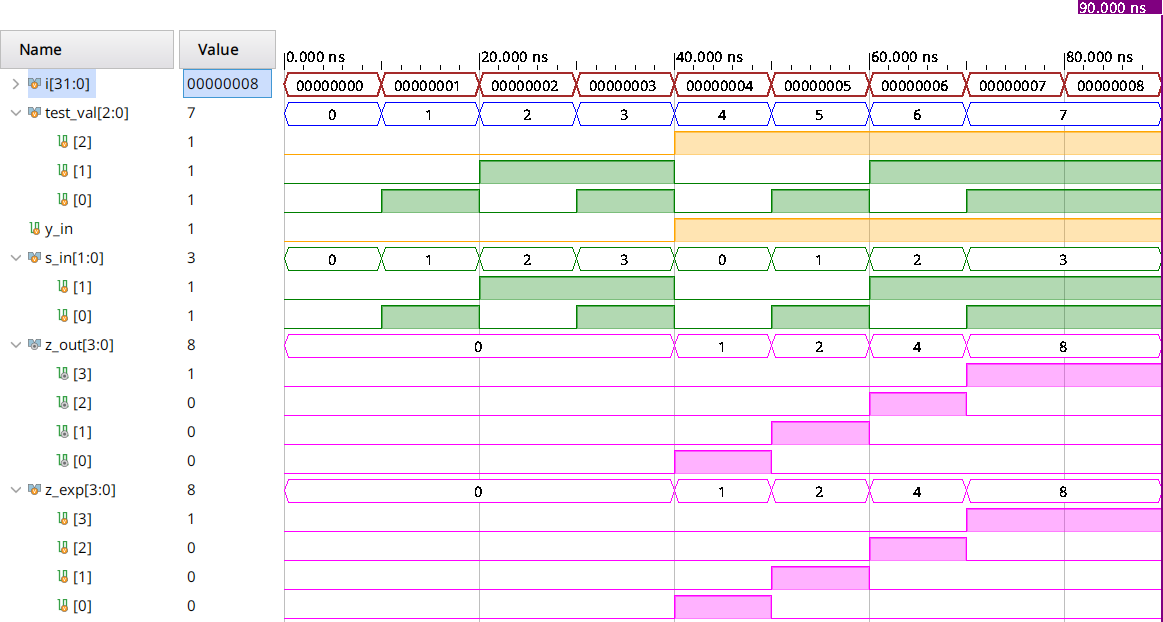
\includegraphics[width=1\textwidth]{../data/test_boe_time_verilog.png}
	\caption{Временная диаграмма тестирования Демультиплексора <<1 в 4>>}
\end{figure}


% -------------------------------

\section*{Выводы по работе}
\addcontentsline{toc}{section}{Выводы по работе}
В данной лабораторной работе были спроектированы и протестированы два цифровых элемента на КМОП-транзисторах: NOR-вентиль и Демультиплексор <<1 в 4>>. Основной целью было изучить их временные характеристики, измерить задержки распространения, рассчитать максимально допустимые рабочие частоты и проверить реализацию на языке System Verilog.

Для \textbf{NOR-вентиля} задержка распространения \( t_{pd} \) была рассчитана как среднее значение между задержками переднего и заднего фронтов, что составило 12.5 \text{ нс}.
Максимальная частота работы NOR-вентиля составила \( 80 \text{ МГц}. \)
Эти данные подтверждают, что NOR-вентиль на КМОП-транзисторах способен работать на высоких частотах, хотя и имеет ограничения, связанные с физическими характеристиками транзисторов.

Для \textbf{Демультиплексора <<1 в 4>>} задержка распространения была определена как теоретически - как сумма задержек по критическому пути, состоящему из четырёх NOR-вентилей, так и эмпирически - по временной диаграмме. Теоретическое значение \( t_{pd} \) для демультиплексора было рассчитано как \( t_{pd} = 4 \cdot t_{pd_{NOR}} = 50 \text{ нс} \). Однако измерения на временной диаграмме показали более высокую задержку в \(103 \, \text{нс}\), максимальная рабочая частота демультиплексора составила: \(9.7 \text{ МГц}.\)

Эта частота значительно ниже, чем у одиночного NOR-вентиля, что объясняется накоплением задержек на критическом пути из-за последовательного соединения вентилей. Полученные результаты демонстрируют, что производительность комбинационной схемы зависит от критического пути — чем больше элементов в пути, тем выше задержка и ниже рабочая частота.

Для описания и тестирования схемы демультиплексора был применён язык System Verilog, который позволил реализовать модули и тестовое окружение. Тестирование показало корректную работу схемы при всех возможных комбинациях входных сигналов, что подтверждает правильность логики и задержек, заложенных в проект.

Полученные в ходе работы результаты подтверждают необходимость учета задержек при проектировании цифровых схем. Максимальная частота, определяемая как обратная величина к задержке критического пути, является ключевым показателем производительности комбинационных схем. Эти результаты также показывают значимость выбора правильной архитектуры для минимизации задержек, особенно в комплексных схемах. Знания, полученные при работе с Verilog и SPICE-моделированием, будут полезны для дальнейших проектов, требующих учета временных характеристик и обеспечения надёжной работы схем на высоких частотах.


% -------------------------------

\end{document}
